\documentclass[11pt]{article}
\usepackage[utf8]{inputenc}
\date{}
\usepackage{amsmath,amssymb,amsfonts, bbm, mathtools}
\usepackage{algorithm,algpseudocode, graphicx}
\usepackage{titlesec, listings, pgfplots}
\usepackage{stackengine, hyperref, float, bm}
\usepackage{tikz}
\usepackage{hyperref}
\usepackage{subfig, pgfplots, tikz, soul, color}
\usepackage[linguistics]{forest}
  \documentclass[border=3pt,tikz]{standalone}
\usepackage{amsmath} % for aligned
%\usepackage{amssymb} % for \mathbb
\usepackage{tikz}
%\usepackage{etoolbox} % for \ifthen
\usepackage{listofitems} % for \readlist to create arrays
\usetikzlibrary{arrows.meta} % for arrow size
\usepackage[outline]{contour} % glow around text
\contourlength{1.4pt}

\tikzset{>=latex} % for LaTeX arrow head 
\usepackage{xcolor}
\colorlet{myred}{red!80!black}
\colorlet{myblue}{blue!80!black}
\colorlet{mygreen}{green!60!black}
\colorlet{myorange}{orange!70!red!60!black}
\colorlet{mydarkred}{red!30!black}
\colorlet{mydarkblue}{blue!40!black}
\colorlet{mydarkgreen}{green!30!black}
\tikzstyle{node}=[thick,circle,draw=myblue,minimum size=22,inner sep=0.5,outer sep=0.6]
\tikzstyle{node in}=[node,green!20!black,draw=mygreen!30!black,fill=mygreen!25]
\tikzstyle{node hidden}=[node,blue!20!black,draw=myblue!30!black,fill=myblue!20]
\tikzstyle{node convol}=[node,orange!20!black,draw=myorange!30!black,fill=myorange!20]
\tikzstyle{node out}=[node,red!20!black,draw=myred!30!black,fill=myred!20]
\tikzstyle{connect}=[thick,mydarkblue] %,line cap=round
\tikzstyle{connect arrow}=[-{Latex[length=4,width=3.5]},thick,mydarkblue,shorten <=0.5,shorten >=1]
\tikzset{ % node styles, numbered for easy mapping with \nstyle
  node 1/.style={node in},
  node 2/.style={node hidden},
  node 3/.style={node out},
}
\def\nstyle{int(\lay<\Nnodlen?min(2,\lay):3)} % map layer number onto 1, 2, or 3
%some pre determined packages
\usepackage[english]{babel}
\usepackage[utf8]{inputenc}
\usepackage[font={small,it}]{caption}
\usepackage[top=0.5in, bottom=1in, left=1.6in, right=1.in]{geometry}
\usepackage[normalem]{ulem}

\hypersetup{
    colorlinks=true,
    linkcolor=blue,
    filecolor=magenta,      
    urlcolor=red,
}
\hypersetup{citecolor=magenta}

%using some bib
\usepackage[backend=biber, sorting=none]{biblatex}

\newcommand*{\blankpage}{%
\vspace*{\fill}
{\centering This page intentionally left blank\par}
\vspace{\fill}}
\makeatletter
\renewcommand*{\cleardoublepage}{\clearpage\if@twoside \ifodd\c@page\else
\blankpage
\thispagestyle{empty}
\newpage
\if@twocolumn\hbox{}\newpage\fi\fi\fi}
\makeatother


\titleformat*{\section}{\Large\bfseries}
\titleformat*{\subsection}{\large\bfseries}
\DeclareRobustCommand{\bbone}{\text{\usefont{U}{bbold}{m}{n}1}}
\DeclareMathOperator{\EX}{\mathbb{E}}

\hypersetup{
    colorlinks=true,
    linkcolor=blue,
    filecolor=magenta,      
    urlcolor=red,
}
\hypersetup{citecolor=magenta}

%using some bib
\usepackage[backend=biber, sorting=none]{biblatex}
\addbibresource{references.bib}



\begin{document}
\newpage
\title{\centerline{\rule{15cm}{4pt}} \vspace*{0.2cm} \textbf{A Brief Introduction to Deep Neural Networks}\vspace*{0.01cm} \\\centerline{\rule{15cm}{2pt}}}
\author{
  Sarper Yurtseven\\
  \texttt{sarperyn@gmail.com}}
\maketitle
{

}


\newpage

\section*{Introduction}
\begin{flushleft}
One should have a basic knowledge of linear algebra and calculus to understand some concepts in neural networks.  If you don't have any prior knowledge,  you can have a basic understanding of systems by looking at my notes on \href{https://github.com/sarperyn/linearalgebra/blob/main/3-Systems-of-LinearEquations/Systems-of-LinearEquations.pdf} {systems of linear equations} and \href{https://github.com/sarperyn/linearalgebra/blob/main/2-MatrixOperations/MatrixOperations.pdf}{matrix operations}. These notes are not complete yet. However, after reading the notes you will have a fundamental knowledge to understand the linear algebraic operations we will be doing. Basic linear algebra is not the only requirement as I mentioned above. I do not have calculus notes but I'm working on them.  If you contact me from anywhere, I'm happy to share some resources for calculus.
\end{flushleft}


\section*{Forward Propagation}

\begin{flushleft}
Assume that we have \textbf{m} examples. Let's review the general formulas we know. 
\end{flushleft}
\begin{flushleft}

$n^{[L]}$: number of units in layer L\\
$A^{[L]} & = \sigma(Z^{[L]})  = \sigma(W^{[L]} \cdot A^{[L-1]} + b^{[L]}) \\ $
$W^{[L]}.shape  = (n^{[L]},n^{[L-1]} )\\ $
$b^{[L]}.shape = (n^{[L]},1 )\\ $
$A^{[L]}.shape  = Z^{[L]}.shape = (n^{[L]},n^{[L-1]} )$



\end{flushleft}


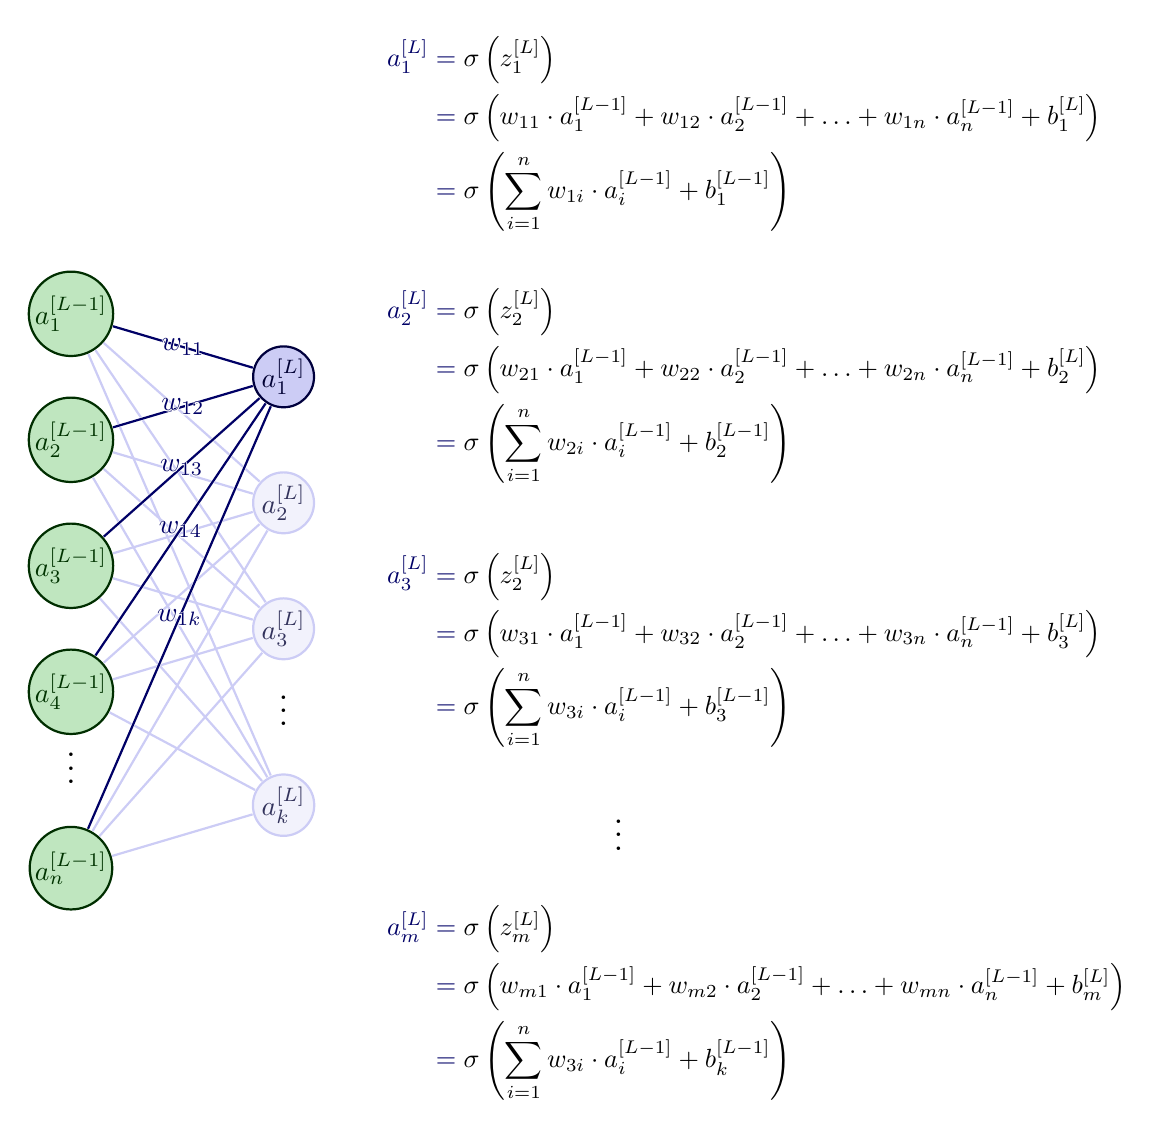
\begin{tikzpicture}[x=2.7cm,y=1.6cm]
  \message{^^JNeural network activation}
  \def\NI{5} % number of nodes in input layers
  \def\NO{4} % number of nodes in output layers
  \def\yshift{0.4} % shift last node for dots
  
  % INPUT LAYER
  \foreach \i [evaluate={\c=int(\i==\NI); \y=\NI/2-\i-\c*\yshift; \index=(\i<\NI?int(\i):"n");}]
              in {1,...,\NI}{ % loop over nodes
    \node[node in,outer sep=0.6] (NI-\i) at (0,\y) {$a_{\index}^{[L-1]}$};
  }
  
  % OUTPUT LAYER
  \foreach \i [evaluate={\c=int(\i==\NO); \y=\NO/2-\i-\c*\yshift; \index=(\i<\NO?int(\i):"k");}]
    in {\NO,...,1}{ % loop over nodes
    \ifnum\i=1 % high-lighted node
      \node[node hidden]
        (NO-\i) at (1,\y) {$a_{\index}^{[L]}$};
      \foreach \j [evaluate={\index=(\j<\NI?int(\j):"k");}] in {1,...,\NI}{ % loop over nodes in previous layer
        \draw[connect,white,line width=1.2] (NI-\j) -- (NO-\i);
        \draw[connect] (NI-\j) -- (NO-\i)
          node[pos=0.50] {\contour{white}{$w_{1 \index}$}};
      }
    \else % other light-colored nodes
      \node[node,blue!20!black!80,draw=myblue!20,fill=myblue!5]
        (NO-\i) at (1,\y) {$a_{\index}^{[L]}$};
      \foreach \j in {1,...,\NI}{ % loop over nodes in previous layer
        %\draw[connect,white,line width=1.2] (NI-\j) -- (NO-\i);
        \draw[connect,myblue!20] (NI-\j) -- (NO-\i);
      }
    \fi
  }
  
  % DOTS
  \path (NI-\NI) --++ (0,1+\yshift) node[midway,scale=1.2] {$\vdots$};
  \path (NO-\NO) --++ (0,1+\yshift) node[midway,scale=1.2] {$\vdots$};
   \path (NO-\NO) --++ (3,-0.7+\yshift) node[midway,scale=1.2] {$\vdots$};
  
  % EQUATIONS
  \def\agr#1{{\color{mydarkgreen}a_{#1}^{(0)}}}
  \node[below=17,right=11,mydarkblue,scale=0.95] at (1.3,3.3)
    {$\begin{aligned} %\underset{\text{bias}}{b_1}
       a_{1}^{[L]} &= \color{black}\sigma\left( \color{black}
       		z_{1}^{[L]}
       		 \color{black}\right)\\
       & = \color{black}\sigma\left( \color{black}
            w_{11} \cdot a^{[L-1]}_{1} + w_{12} \cdot a^{[L-1]}_{2} + \ldots + w_{1n} \cdot a^{[L-1]}_{n} + b_1^{[L]}
          \color{black}\right)\\
       & = \color{black}\sigma\left( \color{black}
            \sum_{i=1}^{n} w_{1i} \cdot a^{[L-1]}_{i} + b_1^{[L-1]}
           \color{black}\right)
     \end{aligned}$};
   \node[below=17,right=11,mydarkblue,scale=0.95] at (1.3,1.3)
    {$\begin{aligned} %\underset{\text{bias}}{b_1}
       a_{2}^{[L]} &= \color{black}\sigma\left( \color{black}
       		z_{2}^{[L]}
       		 \color{black}\right)\\
       & = \color{black}\sigma\left( \color{black}
            w_{21} \cdot a^{[L-1]}_{1} + w_{22} \cdot a^{[L-1]}_{2} + \ldots + w_{2n} \cdot a^{[L-1]}_{n} + b_2^{[L]}
          \color{black}\right)\\
       & = \color{black}\sigma\left( \color{black}
            \sum_{i=1}^{n} w_{2i} \cdot a^{[L-1]}_{i} + b_2^{[L-1]}
           \color{black}\right)
     \end{aligned}$};
  \node[below=17,right=11,mydarkblue,scale=0.95] at (1.3,-0.8)
    {$\begin{aligned} %\underset{\text{bias}}{b_1}
       a_{3}^{[L]} &= \color{black}\sigma\left( \color{black}
       		z_{2}^{[L]}
       		 \color{black}\right)\\
       & = \color{black}\sigma\left( \color{black}
            w_{31} \cdot a^{[L-1]}_{1} + w_{32} \cdot a^{[L-1]}_{2} + \ldots + w_{3n} \cdot a^{[L-1]}_{n} + b_3^{[L]}
          \color{black}\right)\\
       & = \color{black}\sigma\left( \color{black}
            \sum_{i=1}^{n} w_{3i} \cdot a^{[L-1]}_{i} + b_3^{[L-1]}
           \color{black}\right)
     \end{aligned}$};
  \node[below=17,right=11,mydarkblue,scale=0.95] at (1.3,-3.6)
    {$\begin{aligned} %\underset{\text{bias}}{b_1}
       a_{m}^{[L]} &= \color{black}\sigma\left( \color{black}
       		z_{m}^{[L]}
       		 \color{black}\right)\\
       & = \color{black}\sigma\left( \color{black}
            w_{m1} \cdot a^{[L-1]}_{1} + w_{m2} \cdot a^{[L-1]}_{2} + \ldots + w_{mn} \cdot a^{[L-1]}_{n} + b_m^{[L]}
          \color{black}\right)\\
       & = \color{black}\sigma\left( \color{black}
            \sum_{i=1}^{n} w_{3i} \cdot a^{[L-1]}_{i} + b_k^{[L-1]}
           \color{black}\right)
     \end{aligned}$};
    

  
\end{tikzpicture}
\subsection*{Getting Matrix Dimensions}
\begin{flushleft}
From above operations we know:
\end{flushleft}

\begin{center}
$w_{11} \cdot a^{[L-1]}_{1} + w_{12} \cdot a^{[L-1]}_{2} + \ldots + w_{1n} \cdot a^{[L-1]}_{n} + b_1^{[L-1]} = z_{1}^{[L]} $\\
$ w_{21} \cdot a^{[L-1]}_{1} + w_{22} \cdot a^{[L-1]}_{2} + \ldots + w_{2n} \cdot a^{[L-1]}_{n} + b_1^{[L-1]} = z_{2}^{[L]} $\\
$w_{31} \cdot a^{[L-1]}_{1} + w_{32} \cdot a^{[L-1]}_{2} + \ldots + w_{3n} \cdot a^{[L-1]}_{n} + b_1^{[L-1]} = z_{3}^{[L]}$\\
$\vdots$ \\
$w_{m1} \cdot a^{[L-1]}_{1} + w_{m2} \cdot a^{[L-1]}_{2} + \ldots + w_{mn} \cdot a^{[L-1]}_{n} + b_1^{[L-1]} = z_{k}^{[L]}$\\
\end{center}

\begin{flushleft}
The equations look like a system of linear equations from linear algebra.  To get the dimensions, we're gonna treat them like it.  Let's rewrite the system as matrices.
\end{flushleft}


\vspace{0.5cm}

\begin{center}
$\left \begin{bmatrix}
        w_{1,1} & w_{1,2} & \ldots & w_{1,n} \\
        w_{2,1} & w_{2,2} & \ldots & w_{2,n} \\
        \vdots  & \vdots  & \ddots & \vdots  \\
        w_{k,1} & w_{k,2} & \ldots & w_{k,n}
      \end{bmatrix} 
\begin{bmatrix}
        a_{1}^{[L-1]} \\[0.3em]
        a_{2}^{[L-1]} \\
        \vdots \\
        a_{n}^{[L-1]}
      \end{bmatrix}} 
	+
	  \begin{bmatrix}
        b_{1}^{[L]} \\[0.3em]
        b_{2}^{[L]} \\
        \vdots \\
        b_{k}^{[L]}
      \end{bmatrix}  
      =
       \begin{bmatrix}
        z_{1}^{[L]} \\[0.3em]
        z_{2}^{[L]} \\
        \vdots \\
        z_{k}^{[L]}
      \end{bmatrix}}   
      \right 
$
\end{center}

\begin{center}

\begin{*equation}
$ \underset{k \times n}{W^{[L]}}  \times \underset{n \times m}{A^{[L-1]}} + \underset{k\times 1}{b^{[L]}} = \underset{k \times m}{\mathrm{Z^{[L]}}} $
\end{*equation}
\end{center}

\vspace{0.5cm}
\section*{Backward Propagation}

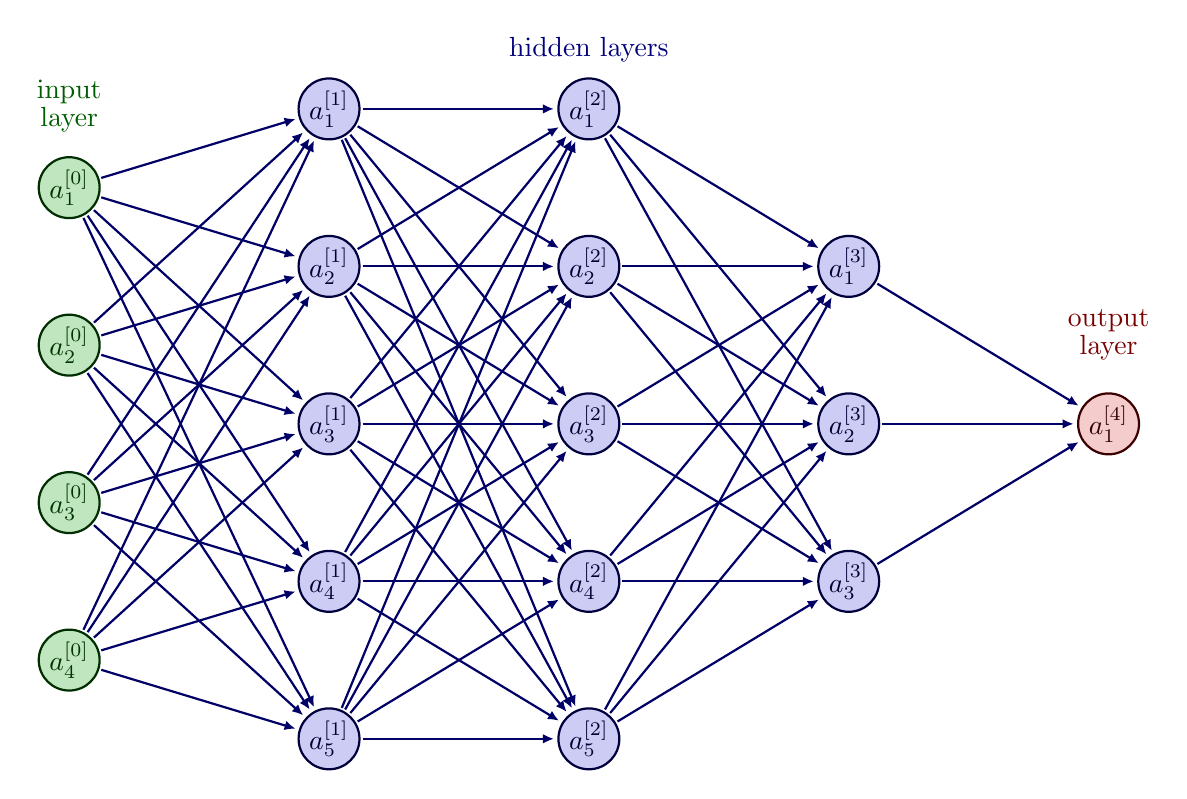
\begin{tikzpicture}[x=3.3cm,y=2cm]
  \message{^^JNeural network with arrows}
  \readlist\Nnod{4,5,5,3,1} % array of number of nodes per layer
  
  \message{^^J  Layer}
  \foreachitem \N \in \Nnod{ % loop over layers
    \edef\lay{\Ncnt} % alias of index of current layer
    \message{\lay,}
    \pgfmathsetmacro\prev{int(\Ncnt-1)} % number of previous layer
    \foreach \i [evaluate={\y=\N/2-\i; \x=\lay; \n=\nstyle;}] in {1,...,\N}{ % loop over nodes
      
      % NODES
      \node[node \n] (N\lay-\i) at (\x,\y) {$a_\i^{[\prev]}$};
      %\node[circle,inner sep=2] (N\lay-\i') at (\x-0.15,\y) {}; % shifted node
      %\draw[node] (N\lay-\i) circle (\R);
      
      % CONNECTIONS
      \ifnum\lay>1 % connect to previous layer
        \foreach \j in {1,...,\Nnod[\prev]}{ % loop over nodes in previous layer
          \draw[connect arrow] (N\prev-\j) -- (N\lay-\i); % connect arrows directly
          %\draw[connect arrow] (N\prev-\j) -- (N\lay-\i'); % connect arrows to shifted node
        }
      \fi % else: nothing to connect first layer
      
    }
    
  }
  
  % LABELS
  \node[above=5,align=center,mygreen!60!black] at (N1-1.90) {input\\[-0.2em]layer};
  \node[above=2,align=center,myblue!60!black] at (N3-1.90) {hidden layers};
  \node[above=8,align=center,myred!60!black] at (N\Nnodlen-1.90) {output\\[-0.2em]layer};
  
\end{tikzpicture}
\vspace{1cm}
\begin{flushleft}
We know that in the first step of backward prop, we're given $dA^{[L]}$. Using $dA^{[L]}$ and the given formulas below, we calculate $dA^{[L-1]},dW^{[L]}$ and $db^{[L]}$.  However, now we gonna just do two of them like we did in the meeting. I'm planning to update this document and add other calculations as well. 
\end{flushleft}
\subsection*{Formulas}
\begin{center}
$dZ^{[L]} = dA^{[L]}  \cdot \sigma(Z^{[L]})$\\
$dW^{[L]} = \frac{1}{m} dZ^{[L]} \cdot A^{[L-1]T}$
\end{center}

\begin{flushleft}
Remember the tree structure. 
\end{flushleft}
\vspace{0.5}
%%Tree structure
\begin{center}

\begin{forest}
  [$ L(A^{4}\, y) $
    [$A^{[4]} = \sigma(Z^{[4]})$
      [$Z^{[4]}$
      	[$W^{[4]} $]
      	[$A^{[3]} $      
        		[$Z^{[3]} $
        			[$W^{[3]} $]
        			[$A^{[2]} $
					[$Z^{[2]}$
						[$W^{[2]}$]
						[$A^{[1]} $
							[$Z^{[1]} $
								[$W^{[1]} $]
								[$A^{[0]} $ ]
								[$b^{[1]} $]							
							]
						]
						[$b^{[2]} $]					
					]        			
        			]
        			[$b^{[3]} $]   
        		]
        	]
      	[$b^{[4]} $]       
    ]         	
  ]      	
]
\end{forest}
\end{center}

\begin{flushleft}
Instead of Andrew's notation, we're gonna use the following notation.
 $\frac{\partial L}{\partial Z^{[L]}} = dZ^{[L]}$,  $\frac{\partial L}{\partial W^{[L]}} = dW^{[L]}$. Now let's take some derivative
\end{flushleft}

\begin{flushleft}


\end{flushleft}

\newpage


\begin{center}
$ \underbrace{\frac{\partial L}{\partial Z^{[4]}} }  =  \underbrace{ \frac{\partial L}{\partial A^{[4]}} \cdot}  \underbrace{\frac{\partial A^{[4]}}{\partial Z^{[4]}}} $
\end{center}
\vspace{1cm}

\begin{center}
$ \underbrace{\frac{\partial L}{\partial Z^{[3]}} }  =  \underbrace{ \frac{\partial L}{\partial A^{[4]}} \cdot \frac{\partial A^{[4]}}{\partial Z^{[4]}}  \cdot \frac{\partial Z^{[4]}}{\partial A^{[3]}} \cdot}  \underbrace{\frac{\partial A^{[3]}}{\partial Z^{[3]}}} $
\end{center}
\vspace{1cm}
\begin{center}
$ \underbrace{\frac{\partial L}{\partial Z^{[2]}} }  =  \underbrace{ \frac{\partial L}{\partial A^{[4]}} \cdot \frac{\partial A^{[4]}}{\partial Z^{[4]}}  \cdot \frac{\partial Z^{[4]}}{\partial A^{[3]}} \cdot \frac{\partial A^{[3]}}{\partial Z^{[3]}} \cdot \frac{\partial Z^{[3]} }{\partial A^{[2]}} }  \underbrace{\frac{\partial A^{[2]}}{\partial Z^{[2]}}} $
\end{center}
\vspace{2cm}

\begin{center}
$ \underbrace{\frac{\partial L}{\partial W^{[4]}} }  =  \underbrace{ \frac{\partial L}{\partial A^{[4]}} \cdot \frac{\partial A^{[4]}}{\partial Z^{[4]}} } \cdot \underbrace{ \frac{\partial Z^{[4]}}{\partial W^{[4]}} }  $
\end{center}
\vspace{1cm}
\begin{center}
$ \underbrace{\frac{\partial L}{\partial W^{[3]}} }  =  \underbrace{ \frac{\partial L}{\partial A^{[4]}} \cdot \frac{\partial A^{[4]}}{\partial Z^{[4]}}  \cdot \frac{\partial Z^{[4]}}{\partial A^{[3]}} \cdot  \frac{\partial A^{[3]}}{\partial Z^{[3]}}} \cdot \underbrace{ \frac{\partial Z^{[3]}}{\partial W^{[3]}}} $
\end{center}
\vspace{1cm}
\begin{center}
$ \underbrace{\frac{\partial L}{\partial W^{[2]}} }  =  \underbrace{ \frac{\partial L}{\partial A^{[4]}} \cdot \frac{\partial A^{[4]}}{\partial Z^{[4]}}  \cdot \frac{\partial Z^{[4]}}{\partial A^{[3]}} \cdot \frac{\partial A^{[3]}}{\partial Z^{[3]}} \cdot \frac{\partial Z^{[3]} }{\partial A^{[2]}}  \cdot  \frac{\partial A^{[2]}}{\partial Z^{[2]}} } \cdot \underbrace{\frac{\partial Z^{[2]}}{\partial W^{[2]}}} $
\end{center}



\end{document}
